\section{The finding of Meridian Way}
\margininbox{Meridian Way}{
     \begin{itemize}
    \item Rhys Tyers
    \item Tanguy Racine
    \end{itemize}}{\explo}

The quest of finding a lower entrance to the system is without any doubt a noble one and hasn't been completed as I write these lines. The \passage{Jetstream} extension of the system was spearing south, well away from the main tangle of passages that make up \passage{Sysmig}. Less than 400\,m to the surface, southwards and upwards, the chances of ending the push by popping out onto the sunlit forest floor were as good as any. In fact, they were better than that: the serendipitous discovery of \passage[cave]{Coincidence Cave} earlier in the week (\vref{sec: coincidence cave}) had revived the belief that the entrance might exist. A draughting hole on the surface, the alignment of a large surface canyon with the underground passage. What are the odds?

\begin{pagefigure}
\checkoddpage \ifoddpage \forcerectofloat \else \forceversofloat \fi
\centering
\frame{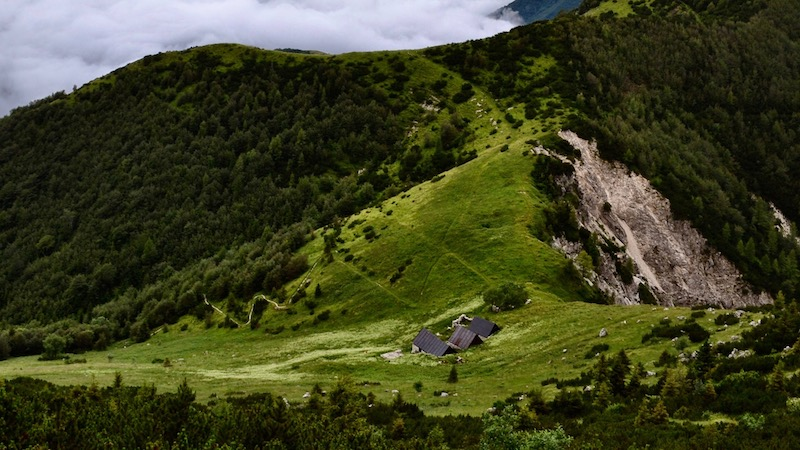
\includegraphics[width=\textwidth]{images/2015/tanguy-meridian-2015/kal-clouds.jpg}}
\caption{Where we hoped to meet the surface, somewhere in the lush landscape below the \protect\passage{Sheperd's Hut} (\protect\passage{Planina Kal}) \pic{Rhys Tyers}}
\label{planina na kalu}
\end{pagefigure}

Rhys and I checked in at camp \passage{X-Ray} for three nights and two pushing days. \bignote{The ambitious plan was to set off smokers at the pushing front, while a party waited for the appearance of red smoke at the surface} thus proving the passage was connected. This would bring us much needed closure.

After an early start, Rhys and I set off from camp, along the now familiar \passage{Kamikaze} extensions, the long silent passages of \passage{Atlantis}. To our left, the offshoot of \passage{We're Not Alone} beckoned. With the limit of exploration so close, we could not help but have a look at it, to assess the feasibility of pushing the lead. The passage first trended east and bent to the south sharply before turning into a flat clean-washed crawl. With the ceiling coming to meet the floor to a tight, awkward flat out squeeze, it was no wonder the lead had been left unpushed. Passage could be seen continuing beyond, but we left it at what it was: a lead for thin people.

It was almost eleven o'clock, we had been caving at a good pace, and the front was half an hour away. We pressed on, past the boulder field leading to \passage{Sic Semper Tyrannis}, along passages named and trodden since the previous year only. At the main junction to \passage{Jericho}, we turned left, upwind, up the rift. I passed the down climb to \passage{Squidgy Goodness} where the corpse of the Creature was, and up the ropes Gergely had rigged in 2014. Rhys disappeared down the next pitch, which was the beginning of \passage{Jetstream} and showed me the way up the climbs.

\begin{figure*}[t!]
\checkoddpage \ifoddpage \forcerectofloat \else \forceversofloat \fi
\centering
\frame{
\includegraphics[width=\textwidth]{images/2015/tanguy-meridian-2015/extended_elevation_south.png}}
\caption{Helpful notes for future \protect\passage{Jetstream} explorers, drawn in the Underground Camp logbook \pen{Rhys Tyers, underground logbook}}
\label{Notebook}
\end{figure*}

At the very apex of surveyed passage of \passage{Jetstream}, the rift split into two routes. One was continuing directly upwards in the same fashion as the ten metre pit we'd just free climbed. The convenient ledges that had brought us this far disappeared quickly and it was deemed unsafe without a rope. Glory would have to wait. Instead, we slid down the slanting rift continuation, down the scree slope to a boulder choke. When \bignote{faced with the pushing front, crowbar in hand and with a clear idea of what was to be done, a smile crept on my face}: that was precisely what I'd signed up for and I was filled with a feeling of endless opportunities.

I levered a block of limestone out of the choke, then pushed two others to the side, and the way on was clear. I wriggled forward, both hands extended in front of me, getting a grip on the boulders on the other side and sat, looking, silent. Rhys followed quickly.

Grinning at the continuation, we stepped off to find the lower entrance. For about 30\,m the dream was on because the cave didn't change nature: it remained an unstable chossy bedding plane descent. I heard Rhys commenting on the lack of easy walking passage.

Almost as an answer to our expectations, the passage opened up almost instantly into a dry, walking height phreatic passage and better still, led to a junction! Rhys quickly stepped to the right, I to the left. The passage on the left twisted down and up before resuming its southern course, but the fault control, pervasive in that part of the cave meant it was going down, ever so slightly towards the west. \bignote{Occasionally I would point out to Rhys where the fault planes were exposed, they were beautifully smooth}.

When the passage wormed its way to the top of a sloping pitch, we knew it was almost a game over for us. We were too deep, or not far enough south to intercept the surface. Descending the pitch meant we had to find more horizontal distance! Still, we decided to descend, first by free climbing the 55$^{\circ}$  slope, using the various ledges covered by white sand. About 5 metres down, the slope increased and it dawned on us that we would have to bolt it.

Having left our rope and bolting kit at the start of the squeeze, we doubled back to retrieve them and set about driving the anchors for a Y-hang. I put in the first one, far above the pitch head as it was easier for a left-handed person. Rhys put in the other, and rigged his descender. Down he went until he reached the stopper knot. \bignote{The end of the pitch was in sight, but the rope was a good ten metres short}. It would also need to be deviated.

We considered our options: there was rope at the junction at the start of \passage[junction]{Jericho}, but the horror of \passage{Jetstream} (\passage{Penitence}-like crawl, loose climb, muddy slope etc.) had to be passed again and again. As it was approaching two o'clock, we resolved to abandon the plan to set off the smokers and instead to simply reach the bottom of the pitch and see what was there.

At \passage[junction]{Jericho} junction, after a soupy-fishy-couscous mix, we retrieved the longer rope and turned back towards the pushing front. At the pitch head, I descended slowly, watching the rope carefully to avoid rub points on the various ledges. I had put a deviation two thirds of the way down which ended up swallowing 5 metres of green tape. This done, my feet touched the floor once more on virgin passage. I stayed silent as Rhys descended.

\begin{map}[t!]
\checkoddpage \ifoddpage \forcerectofloat \else \forceversofloat \fi
\centering
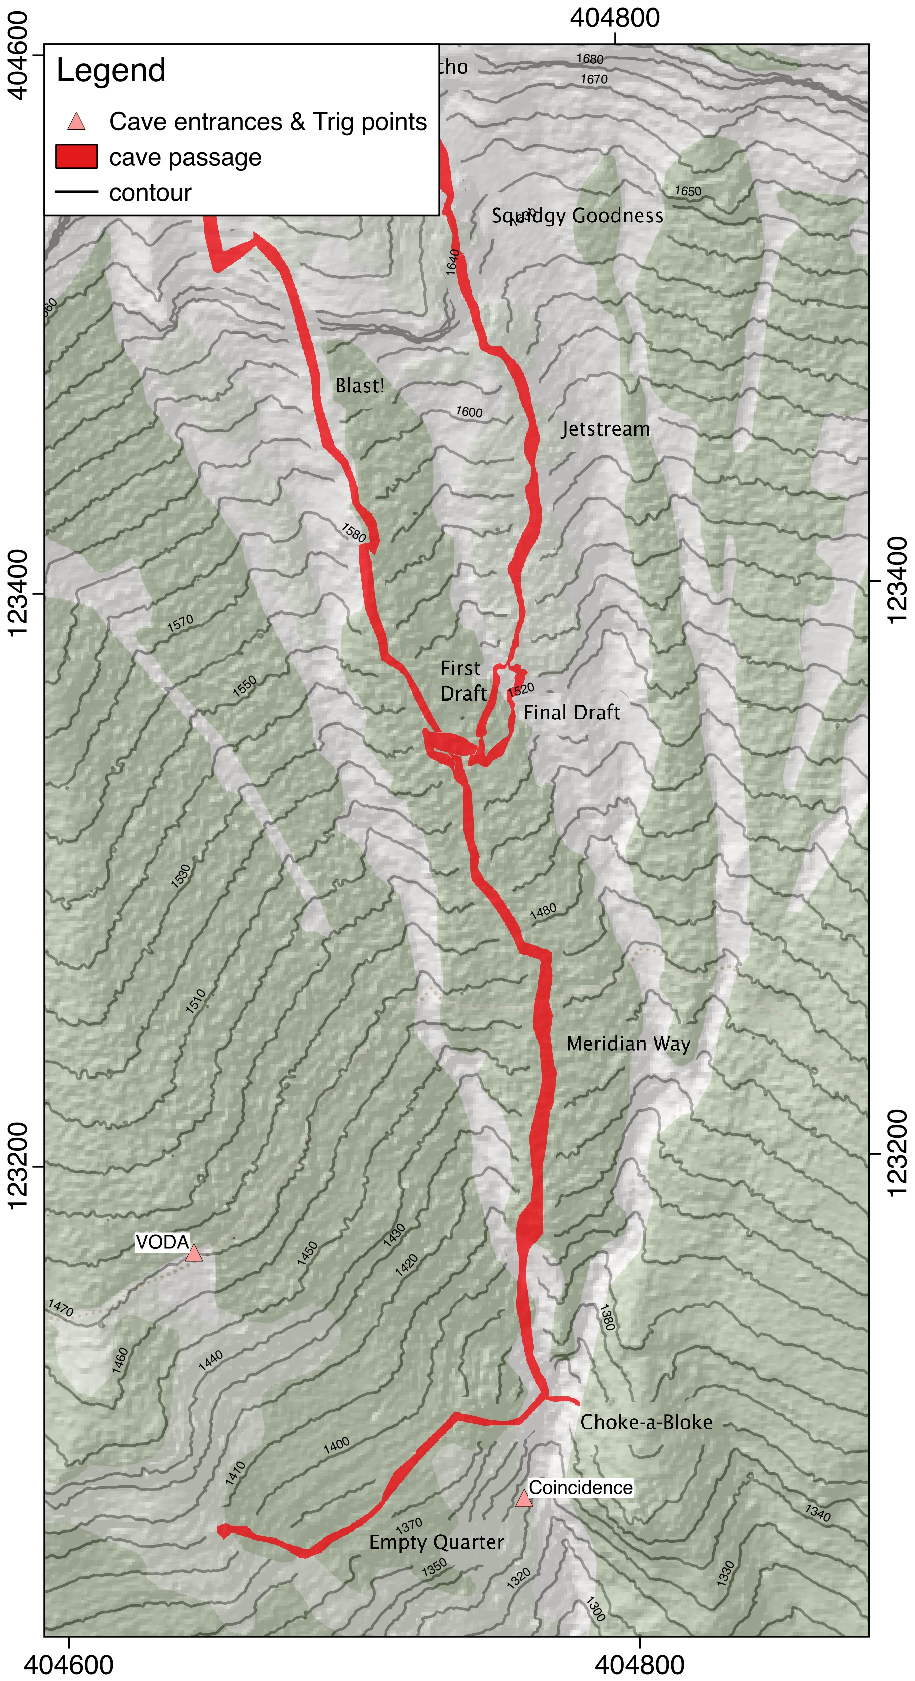
\includegraphics[width=\textwidth]{images/2015/tanguy-meridian-2015/meridian_map.pdf}
\caption[Meridian way topographic map]{Topographic map with superimposed cave passage showing the \protect\passage{Atlantis} extensions heading towards the surface, and in all probability a dormouse sized entrance at least. Interestingly, the fault controlled passages of \protect\passage{First Draft} and the \protect\passage{Final Draft} pitch line up with a conspicuous surface canyon, running down the face of \protect\passage[mountain]{Migovec}, in which \protect\passage{Coincidence Cave} was found --- Slovenian National Grid, EPSG 3794}
\label{map:meridianmap}
\end{map}


Below the pitch, the passage opened up, intercepting a $5\times2$\,m horizontal passage trending south. This was our way to the surface \mapref{map:meridianmap}! Then followed the best minutes of exploration along a seemingly endless horizontal passage. I thought of \passage{Atlantis}, of \passage{Friendship Gallery}, of all the reports, stories, tales even, of glorious easy walking passage and felt immense pride in walking alongside Rhys in this gallery.

Along the way, \bignote{we noted several interesting features: bits of hair, excrements, scratch marks}, bones! It was all there, the proof that mammals of some sort have been here before. To the best of my knowledge, the Creature is trogloxene, its presence only explained by the ease with which it could move from a lower entrance to this passage. Indeed, the fact that one could have made its way to \passage{Hawaii} doesn't seem as remotely incredible as it once did. The majority of passage from the end of our gallery to \passage{Hawaii} is simply horizontal!

\begin{survey*}[t!]
\checkoddpage \ifoddpage \forcerectofloat \else \forceversofloat \fi
\includegraphics[width = \linewidth]{"images/2015/tanguy-meridian-2015/coincidence".png}
\caption[Aven view of Empty Quarter]{The following view shows the closest approach between \protect\passage{Empty Quarter} and the surface to be $\approx$280\,m --- produced on \emph{Aven}}
\end{survey*}

We turned round and surveyed the `\passage{Meridian Way}' when a boulder choke prevented the easy walking. The passage goes on - to the lower exit - it must! Back at the pitch base, the passage also disappeared into darkness towards the north. Another long gallery! We would have to wait for another team to explore this particular passage, as for us time pressed on: this was the beginning of a long survey, and an even longer return journey.

\name{Tanguy Racine}



\section{Pushing our Luck above Cuckoo's Nest}
\margininbox{Push Your Luck}{
     \begin{itemize}
    \item Rhys Tyers
    \item Tanguy Racine
    \end{itemize}}{\explo}
    
We'd overslept a lot I decided as I saw that it was already past ten o'clock. It did not surprise me, since we'd only come back from \passage{Meridian Way} just before midnight. Then we'd collapsed into bed.
 In the darkness of the tent I sat upright in the snug sleeping bag, furry hat on. My breath turned to a silvery mist by the light of my headtorch. The fairy lights had dimmed so much I could hardly make them out. I left the comfort and warmth of the Nitestar 450, put on the largest crocks I could find, and lit the church candles. One, two, three dancing lights.

`Where are we going to push then' I asked Rhys, whilst tucking into a rich soupy couscous mix.
`I know of a lead Clare pushed in 2013, up \passage{Cuckoo's Nest}' he replied.
`I've never been down that way. How do you get to the passage? Is it past the traverse at the top of \passage{Big Rock Candy Mountain}'
`Yeah, that's it, you traverse and then drop into a chamber. There'll be a rope on your right, the one from \passage{Euphrates}. It's a grim bit of cave, which is why no one's ever gone back to retrieve the rope after surveying. It connects back to \passage{Xanadon't} and the hole in \passage{Friendship Gallery}.'
`Fascinating, so fairly close to camp then. Shall we?'
`I'm going to put our call out as 7.00\,pm then'.

 \begin{marginfigure}
\checkoddpage \ifoddpage \forcerectofloat \else \forceversofloat \fi
\centering
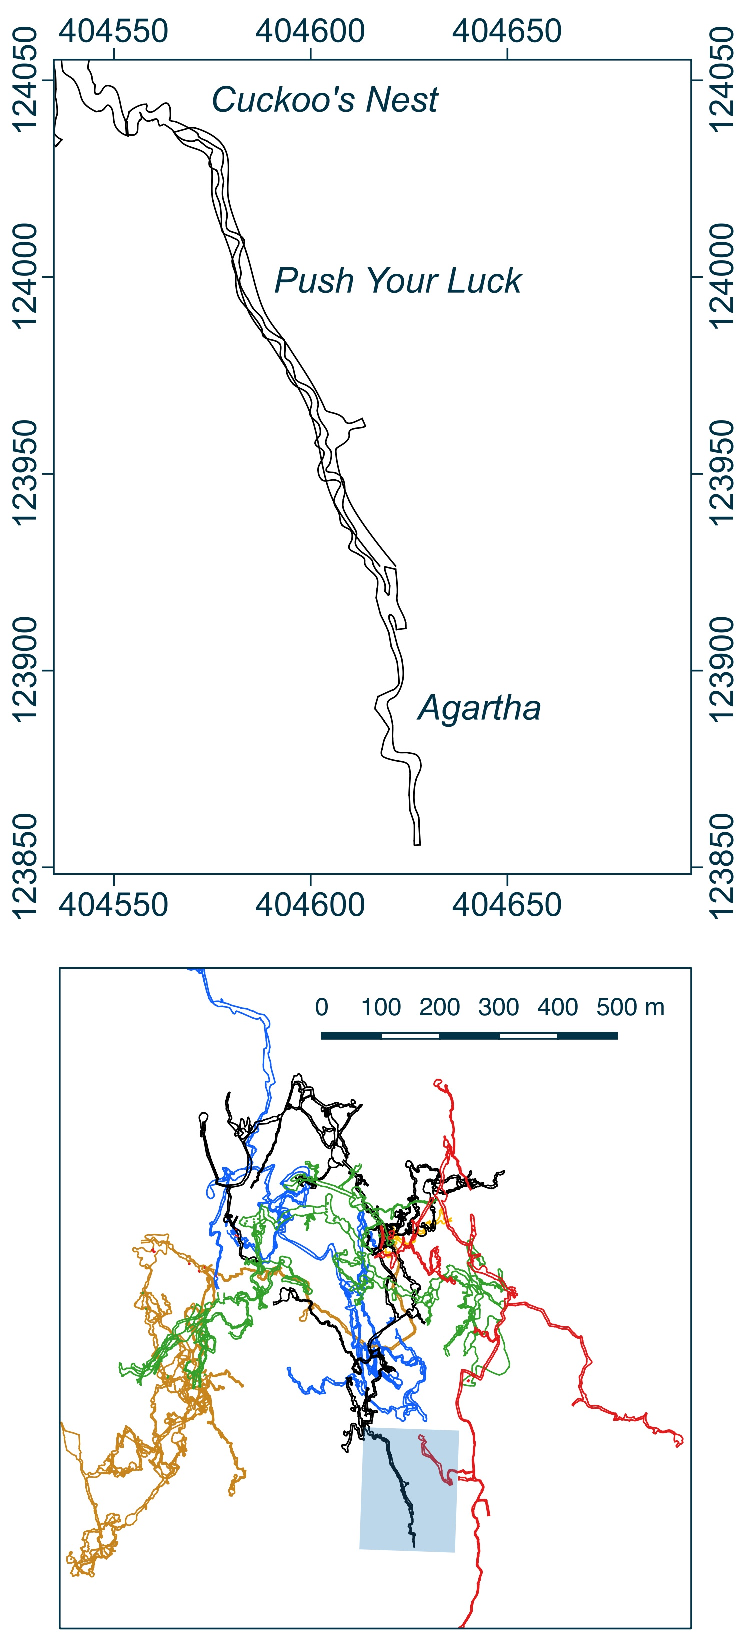
\includegraphics[width= \linewidth]{images/little_insets/push_your_luck_inset.pdf}
 \caption*{Plan view of the \protect\passage[extensions]{Cuckoo's Nest} extensions, Slovenian National Grid ESPG 3794}
 \label{push your luck inset}
\end{marginfigure}

Half an hour later, we left camp, along \passage{Friendship Gallery}, towards the head of \passage{Big Rock}. There we kept to the right, traversed on the muddy pitch head, until a short succession of small hangs brought us into a chamber overlooking the massive drop. After a small climb down, we followed a sinuous muddy rift until we had to climb up again using a greasy in situ rope. From then on, the rumble of flowing water could be heard distinctly, and we soon came upon a fork in the passage, with the way to \passage{Straight Jacket} and \passage{Rejuvenation Rift} to our right. The way on to the end of \passage{Cuckoo's Nest} was to the left, with the passage descending slightly until we reached the water at the bottom of the rift.


Past a few meanders, the rift widened to an oval shape and a cascade three metres high draped the far wall. A PSS was left underneath a egg like pure white limestone cobble: \passage{Cuckoo's Nest} station 3. Rhys and I contemplated the pushing front. The only viable way on was up, and could be reached by bridging our way up, away from the water. Several ledges were seen to protrude, giving steady footholds about two and a half metres from the floor. Feet and back against the scalloped walls, Rhys  climbed up gracefully and I followed.

At the first ledge I started removing the majority of loose rocks I could reach, while Rhys gained more height. Ledge by ledge we climbed until we reached the top of the traverse, dry, muddy, and loose. There we steadily traversed in the upstream direction, until we dropped into the streamway again. We were faced with a similar second climb. Further traverse enabled us to gain the top of third cascade, after which we continued almost a stream level on a meandering rift heading steadily southward.

 \begin{marginfigure}
	\checkoddpage \ifoddpage \forcerectofloat \else \forceversofloat \fi
	\centering
	\frame{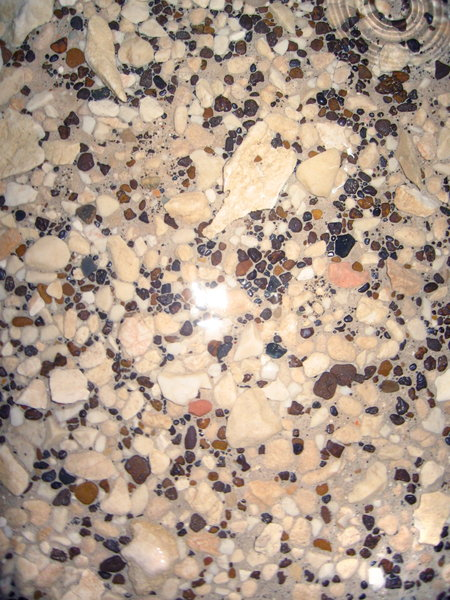
\includegraphics[width=\linewidth]{images/2015/tanguy-push-2015/pebbles_in_alchemy_jana_carga.jpg}}
	\caption{Pebbles similar to those found in \protect\passage{Push Your Luck} streamway can also be seen at the bottom of \protect\passage{Alchemy} pitch in the entrance series of \protect\passage{Vrtnarija} \pic{Jana \v{C}arga}}
	\label{push your luck pebbles}
\end{marginfigure}

Our progress was not hampered by any further climbs or constrictions, and soon I lost count of the twists and turns. We arrived a boulder collapse. Navigating our way in the vertical maze we eventually reached the roof again, but to our surprise, a flat out crawl lead off back in the opposite direction. Instead of following it we negotiated the way past the collapse, and regained the stream. From then on, the rift enlarged particularly on the occasion of three meanders, where the base was very much wider, the stream lazier and where sediments had deposited on the shelves: granules and small pebbles of white limestone and black haematite. This was a delightful sight, the finest photogenic cave sediments I'd seen on \passage{Migovec} yet!

After the meanders, the rift resumed its course and after a further collapse Rhys and I called it day. This was more than enough rift to survey. Doubling back to the start of the passage to get survey paper and instruments, we tried to gauge the length of our find. With the 350\,m discovered a day earlier at \passage{Meridian Way}, would we reach the 500\,m of passage found in one camping trip'


As I took the survey notebook and pencil, I stuffed my gloves inside my oversuit, and we started the survey. After the climbs, we started the meanders. As I sat, writing down the lengths and angles Rhys dictated the gloves fell down to my navel and made a noticeable bulge underneath the suit.
\bignote{`Tanguy, are these your gloves, or are you just happy to see me?'} asked Rhys.
`It's the passage' I answered, and we both had a good laugh.

After fifty or so survey legs, we arrived at the boulder collapse. I ate a chocolate bar while my partner in crime added up the legs. `About 250\,m in the book, what a lovely tourist trip - that's what you call pushing one's luck'.

\name{Tanguy Racine}

\begin{survey}[b!]
\checkoddpage \ifoddpage \forcerectofloat \else \forceversofloat \fi
\centering
\frame{\includegraphics[width=\textwidth]{"images/2015/tanguy-push-2015/push_your_luck".png}}
\caption{The plan view of the \protect\passage{Push your Luck} streamway, an active undergound stream which journeys northward all the way to \protect\passage{Highway 32} \pen{Tanguy Racine, underground logbook}}
\label{map:pushyourluck}
\end{survey}
